%; whizzy paragraph -pdf xpdf -latex ./whizzypdfptex.sh
%; whizzy-paragraph "^\\\\begin{frame}\\|\\\\emtext"
% latex beamer presentation.
% platex, latex-beamer $B$G%3%s%Q%$%k$9$k$3$H$rA[Dj!#(B 

%     Tokyo Debian Meeting resources
%     Copyright (C) 2012 Junichi Uekawa

%     This program is free software; you can redistribute it and/or modify
%     it under the terms of the GNU General Public License as published by
%     the Free Software Foundation; either version 2 of the License, or
%     (at your option) any later version.

%     This program is distributed in the hope that it will be useful,
%     but WITHOUT ANY WARRANTY; without even the implied warreanty of
%     MERCHANTABILITY or FITNESS FOR A PARTICULAR PURPOSE.  See the
%     GNU General Public License for more details.

%     You should have received a copy of the GNU General Public License
%     along with this program; if not, write to the Free Software
%     Foundation, Inc., 51 Franklin St, Fifth Floor, Boston, MA  02110-1301 USA

\documentclass[cjk,dvipdfm,12pt]{beamer}
\usetheme{Tokyo}
\usepackage{monthlypresentation}

%  preview (shell-command (concat "evince " (replace-regexp-in-string "tex$" "pdf"(buffer-file-name)) "&")) 
%  presentation (shell-command (concat "xpdf -fullscreen " (replace-regexp-in-string "tex$" "pdf"(buffer-file-name)) "&"))
%  presentation (shell-command (concat "evince " (replace-regexp-in-string "tex$" "pdf"(buffer-file-name)) "&"))

%http://www.naney.org/diki/dk/hyperref.html
%$BF|K\8l(BEUC$B7O4D6-$N;~(B
\AtBeginDvi{\special{pdf:tounicode EUC-UCS2}}
%$B%7%U%H(BJIS$B7O4D6-$N;~(B
%\AtBeginDvi{\special{pdf:tounicode 90ms-RKSJ-UCS2}}

\title{$BEl5~%(%j%"(BDebian$BJY6/2q(B}
\subtitle{$BBh(B94$B2s(B 2012$BG/(B11$B7nEY(B}
\author{$B>e@n=c0l(B\\dancer@debian.org}
\date{2012$BG/(B11$B7n(B17$BF|(B}
\logo{
\includegraphics[width=8cm]{image200607/openlogo-light.eps}}

\begin{document}

\frame{\titlepage{}}

\begin{frame}{$B@_1D=`Hw$K$46(NO$/$@$5$$!#(B}
$B2q>l@_1D$h$m$7$/$*$M$,$$$7$^$9!#(B
\end{frame}

\begin{frame}{Agenda}
\begin{minipage}[t]{0.45\hsize}
  \begin{itemize}
  \item $BCm0U;v9`(B
	\begin{itemize}
	 \item $B0{?)6X;_(B
	 \item $B=!656X;_(B
	 \item $B1DMx3hF06X;_(B
	\end{itemize}
   \item $B:G6a$"$C$?(BDebian$B4XO"$N%$%Y%s%HJs9p(B
	\begin{itemize}
        \item $BBh(B93$B2s(B $BEl5~%(%j%"(BDebian$BJY6/2q(B
	\end{itemize}
   \item DWN quiz
   \item $B;vA02]Bj>R2p(B
 \end{itemize}
\end{minipage} 
\begin{minipage}[t]{0.45\hsize}
 \begin{itemize}
  \item systemd
  \item perf
  \item bluetooth tethering
 \end{itemize}
\end{minipage}
\end{frame}


\section{DWN quiz}
\emtext{DWN quiz}
\begin{frame}{Debian $B>o<1%/%$%:(B}

Debian $B$N>o<1!"$b$A$m$sCN$C$F$^$9$h$M(B?
$BCN$i$J$$$J$s$FCQ$:$+$7$/$F!"CN$i$J$$$H$O8@$($J$$$"$s$J$3$H$d$3$s$J$3$H!"(B
$B$_$s$J$G3NG'$7$F$_$^$7$g$&!#(B

$B:#2s$N=PBjHO0O$O(B\url{debian-devel-announce@lists.deban.org},
\url{debian-devel@lists.deban.org} $B$KEj9F$5$l$?(B
$BFbMF$H(BDebian Project News$B$J$I$+$i$G$9!#(B

\end{frame}

\subsection{$BLdBj(B}
%; whizzy-master ../debianmeetingresume201211.tex
% $B0J>e$N@_Dj$r$7$F$$$k$?$a!"$3$N%U%!%$%k$G(B M-x whizzytex $B$9$k$H!"(Bwhizzytex$B$,MxMQ$G$-$^$9!#(B
%

\santaku
{FTP master $B$K$"$?$i$7$/;22C$7$?$N$O(B}
{iwamatsu}
{ansgar}
{bdale}
{B}
{Ansgar $B$,?7$7$/;22C$7$^$7$?!#(Bmhy, joerg, ansgar $B$N;0?MBN@)$K(B}

\santaku
{pdiff$B$G2?$,2~A1$5$l$?$+(B}
{$B:GBg(B2$B$D$N(BDiff$B$r%@%&%s%m!<%I$9$l$PNI$$$h$&$KJQ99$K$J$C$?(B}
{$B0lF|(B10$B8D$E$D(BDiff$B$r@8@.$9$k$h$&$K$J$C$?(B}
{Diff$B$C$F$J$K$=$l$*$$$7$$$N!)(B}
{A}
{apt-get update $B$NCY$5$,%^%7$K$J$j$^$9$M!#(B}

\santaku
{CTTE 573745 $B$G2?$,7hDj$5$l$?$+(B}
{Mattias Klose $B%/%S(B}
{python $B=*N;$N$*CN$i$;(B}
{$B$_$s$JCgNI$/$7$h$&$M(B}
{C}
{python $B$N%a%s%F%J$N%3%_%e%K%1!<%7%g%sITB-$K$D$$$F$N5DO@$O7k6I$_$s$JCgNI(B
$B$/$7$^$7$g$&$H$$$&7kO@$K$J$j$^$7$?$M!#(B}

\santaku
{$B?7$7$/(BFront Desk$B$N%a%s%P!<$K$J$C$?$N$O(B}
{Kouhei Maeda}
{Iwamatsu}
{Jonathan Wiltshire}
{C}
{4$B?M$K$J$j$^$7$?!'(B
 Bernd Zeimetz      (bzed)
 Enrico Zini        (enrico)
 Jan Hauke Rahm     (jhr)
 Jonathan Wiltshire (jmw)
}

\santaku
{debian installer 7.0 beta3 $B$N?75!G=$G$O$J$$$N$O$I$l$+(B}
{ipv6}
{UEFI}
{grub2}
{C}
{}

\santaku
{}
{}
{}
{}
{}
{}
\santaku
{}
{}
{}
{}
{}
{}
\santaku
{}
{}
{}
{}
{}
{}
\santaku
{}
{}
{}
{}
{}
{}


\emtext{$B;vA02]Bj(B}
{\footnotesize
 %; whizzy-master ../debianmeetingresume201211.tex
% $B0J>e$N@_Dj$r$7$F$$$k$?$a!"$3$N%U%!%$%k$G(B M-x whizzytex $B$9$k$H!"(Bwhizzytex$B$,MxMQ$G$-$^$9!#(B
%

\begin{prework}{ koedoyoshida }

\begin{itemize}
 \item Wheezy$B%$%s%9%H!<%i$N%Q!<%F%#%7%g%s9=@.;~$N%G!<%?>C5nBT$A;~4V!#(B
 $B0E9f2=%Q!<%F%#%7%g%s$r:n$m$&$H$9$k$H2L$F$7$J$/BT$?$5$l$k!#(B
 \item 
 Wheezy$B$NJI;f!#$$$1$F$J$$46$8$G(BOSC$B$H$+$NE8<($GE,Ev$J$b$N$rA*$V$N$,LLE]$G7k6I(Bsqueeze$B$d(BDebian$B$N(B($B2a5n$N(B)$B%8%'%M%j%C%/$J$b$N$rA*$V$3$H$K(B...
 \item 
 $B%G%P%C%0%7%s%\%k$r4^$s$@%P%$%J%j$,$J$$!#(B
 $B0JA0BgE}0l$G4d>>$5$s$,H/I=$7$F$$$?OC$,?J$s$G$$$k$H$&$l$7$$!#(B
\end{itemize}

\end{prework}

\begin{prework}{ $B%-%?%O%i(B }

$B;d$,;HMQ$9$kHO0O$G$O$"$j$^$;$s!#(B

\end{prework}

\begin{prework}{ MATOHARA }

$B$"$^$j;W$$$D$+$J$$$G$9$,!"?M$HOC$r$7$F$$$k$H$-0J2<$N$h$&$J$3$H$r8@$o$l$?$3$H$,$"$j$^$9!#(B
\begin{itemize}
 \item 
 Debian$B$O5,DjCM$N@_Dj$,$$$1$F$J$$$N$G@_Dj$rBt;3$$$8$i$J$$$H1?MQ=PMh$J$/$F9)?t$,L5BL$K3]$+$k(B
 \item 
 Debian$B$O%$%s%9%H!<%k$,Fq$7$$(B
\end{itemize}
$B6qBNNc$rJ9$1$J$+$C$?$N$G$9$,!"@_Dj$K$D$$$F$O@i:9K|JL$J$N$G$=$N?M$K$H$C$F(B
 $B8~$$$F$$$J$+$C$?$+$i$H8@$C$F%@%a$+$H$$$&$H$=$&$G$O$J$$$H;W$$$^$9!#(B
$B$7$+$7!"(BopenSUSE $B$N(BYaST $B$O0l85E*$K4IM}$G$-$FJXMx$=$&$@$J$H$O;W$$$^$9!#(B
$B%$%s%9%H!<%k$,Fq$7$$$H$$$&$N$b@N$N%$%a!<%8$J$N$+8=:_$N$3$H$r8@$C$F$$$k$NITL@$J$N$G$9$,!"%G%9%/%H%C%W8~$1$N%G%#%9%H%j%S%e!<%7%g%s$KHf$Y$k$HA*Br;h$,B?$$$N$GFq$7$/46$8$i$l$k$N$+$b$7$l$^$;$s!#(B

\end{prework}

\begin{prework}{ $BNkLZ?rJ8(B }

$B8=:_$O2~A1$7$F$$$k$+$b$7$l$^$;$s$,!"0lIt(Bkernel$B$N%Q%C%1!<%8$K$h$C$F$O(Bdbg$B%Q%C%1!<%8$,L5$$$b$N$,$"$C$?$j$7$F!":$$C$?7P83$,$"$j$^$7$?!#(B
\end{prework}

\begin{prework}{ $BLnEg!!5.1Q(B }

Debian$B$G$$$1$F$$$J$$5!G=!?<BAu$H$$$o$l$k$H!"(B

\begin{itemize}
 \item  ifupdown$B%Q%C%1!<%8(B
 \item  Solaris10$B0J>e$G$$$&$H$3$m$N(BFMD$B$H$+!"(BSVC$BM_$7$$!#(B
 \item  $B%$%s%9%H!<%i$G(B'/'$BA4It(BBTFS$B$H$$$&$NA*Br2DG=$G$7$?$C$1!)(B
 \item  WEB$BMm$_$G!":G?7(BWEB$B3+H/4X780l<0$N%Q%C%1!<%8%j%]%8%H%j$H$$$&$N$,M_$7$$5$$,$9$k!J(BWEB$B%7%9%F%`$GN.9T$j$b$N$d$i!"NI$/;H$o$l$F$$$=$&$J%P!<%8%g%s$N%=%U%H$KFC2=$7$?%j%]%8%H%j!#$=$l$J$i(Bexperimental$B$7$+B8:_$7$J$$$H$+$G$b%$%$!*!K(B
 \item  Debian$B$H$O$A$g$C$H%:%l$F$k$+$b$7$l$^$;$s$,!"(Bsynaptic$B$O(B...iTunes$B$_$?$$$K$J$C$F$[$7!<(B
\end{itemize}

$B$H8@$$$?$$J|Bj8@$C$F$_$?!#(B
\end{prework}

\begin{prework}{ $B>e@n=c0l(B }

Android $BMQ$N(BADB$B%3%^%s%I$H$+$,I8=`$GF~$C$F$$$k$H4r$7$$$J$!!#(B
\end{prework}

\begin{prework}{ yamamoto }

Debian $B$NM}A[$H?.G0$OBg9%$-$J$s$G$9$,!">/$75$$K$J$kE@$b$"$j$^$9!#(B

$BNc$($P(B Debian-Installer $B$K$O(B non-free $B$GHRI[$5$l$F$$$k(B firmware $B%Q%C%1!<%8$,4^$^$l$F$$$J$$E@$J$I$G$9!#(Bnon-free $B$N%Q%C%1!<%8$O!"MM!9$JM}M3$G(B non-free $B$KJ,N`$5$l$F$$$k$o$1$G$9$,!"$=$N0l$D$K%F%-%9%H$N%=!<%9$,B8:_$7$J$$$?$a!"$H$+$$$&M}M3$b$"$j$^$9!#(B

$BJL$K!V(Bnon-free $B$K$9$k$J!W$H$+<gD%$7$?$$$o$1$G$O$J$$$N$G$9$,!"HRI[$N@)8B$NL5$$%Q%C%1!<%8$^$G!V(Bnon-free $B$@$+$i!W$H!"<}O?$r5q@d$9$k$N$O>/!9$d$j$9$.$G$O$J$$$+$H9M$($F$$$^$9!#(B
\end{prework}

\begin{prework}{ $BLn<s(B }

\begin{itemize}
 \item $B%Q%C%1!<%8$N%j%9%H%"$K(Bdpkg --get-selections$B$O$A$g$C$HHyL/(B
 \item aptitude-run-state-bundle$B$O$$$^$$$AMQES$,$o$+$i$J$$(B
 \item stable$B$K$?$^$K;H$$J*$K$J$i$J$$%Q%C%1!<%8$,$"$k(B
       \begin{itemize}
	\item $B8E$9$.$k$+$i$H$+(B($BNc(B: lxc)
       \end{itemize}

 \item $B%Q%C%1!<%8$N%H%i%s%6%/%7%g%s$,M_$7$$(B
       \begin{itemize}
	\item $B0lEY%$%s%9%H!<%k$7$F$_$F$*$+$7$+$C$?$i(Brevert
	\item $BLdBj$J$1$l$P(Bcommit$B$_$?$$$J(B
       \end{itemize} 
\item multiarch$B$OF3F~$7$FK\Ev$KNI$+$C$?$N$+(B?
\end{itemize}

\end{prework}

\begin{prework}{ $BF|HfLn(B $B7<(B }

$B;H$$$3$_$,B-$j$F$J$$$N$+$b$7$l$^$;$s$,!"(B
$BMzNr4IM}%7%9%F%`$KJ]B8$5$l$F$$$k(Btree$B$r(B
debian$B%Q%C%1!<%8$H$7$F(B build $B$7$?$j(B
install $B$7$?$j$9$k$H$-$KJXMx$J%D!<%k$,(B
$B$"$^$jL5$$$N$+$b$H;W$$$^$7$?!#(B

\end{prework}

\begin{prework}{ dictoss($B?yK\!!E5=<(B) }

iptables$B$N%3%^%s%I0z?t$,B>$N(BOS$B$H0c$&$h$&$J46$8$,$9$k!#$=$N$?$a(Biptables$B$N=i?4<T$,(Bweb$B$GD4$Y$?%3%^%s%I$r<B9T$7$F$b9=J8%(%i!<$G$O$8$+$l$F?I$$!#(B
\end{prework}

}

\emtext{bluetooth tethering}

\begin{frame}{tethering}
\begin{itemize}
 \item Tethering$B$H$O!"7HBSEEOC$NDL?.5!G=$r;H$C$F%Q%=%3%sDL?.$r$9$k$3$H(B
 \item USB$B!"(BWiFi$B!"(BBluetooth$B7PM3$G@\B3$7$F%9%^!<%H%[%s7PM3$G%$%s%?!<%M%C(B
       $B%H@\B3$r$9$k$3$H(B
 \item $BNc!'(B Pocket WiFi
\end{itemize} 
\end{frame}

\begin{frame}{bluetooth $B$H$$$&Kb7"(B}
PAN vs DUN
\end{frame}

\begin{frame}{Bluetooth Tethering}
 Android $B7HBS$G$N@_Dj(B
 \begin{center}
  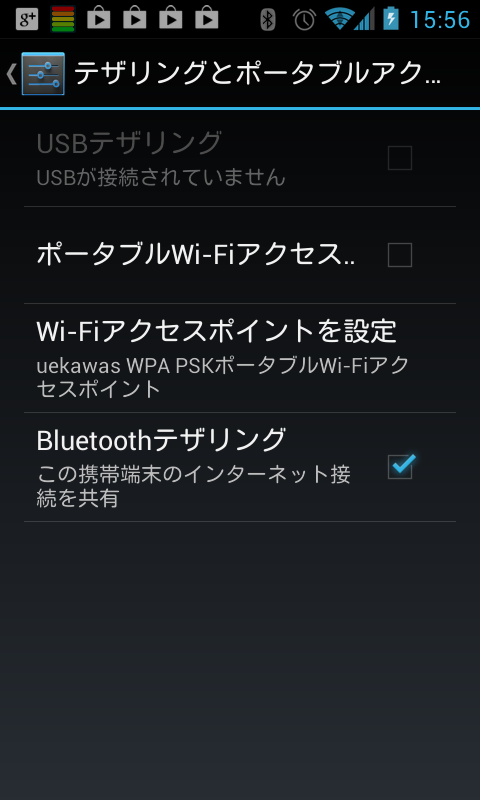
\includegraphics[width=0.3\hsize]{image201211/bt-android.png}
 \end{center}
\end{frame}

\begin{frame}{gnome bluetooth $B@_Dj(B}
 $B%Q%=%3%sB&$H$N%Z%"%j%s%0$,I,MW$G$9(B

 \begin{center}
  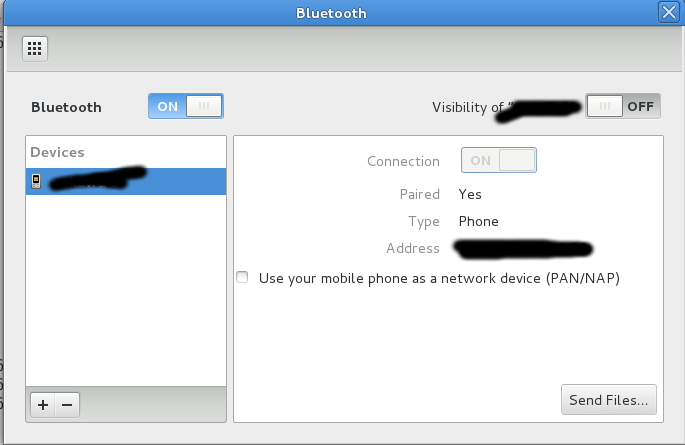
\includegraphics[width=0.5\hsize]{image201211/bt2.png}
 \end{center}
\end{frame}  

\begin{frame}{Bluetooth $B7PM3$G$N@\B3(B}

 \begin{center}
 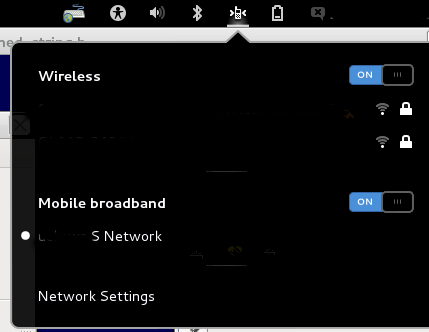
\includegraphics[width=0.5\hsize]{image201211/bt1.png}
 \end{center}
\end{frame}

\begin{frame}[containsverbatim]{bnep0 $B%M%C%H%o!<%/(B}
\begin{commandline}
bnep0     Link encap:Ethernet  HWaddr 
          inet addr:192.168.46.43  Bcast:192.168.46.255  Mask:255.255.255.0
\end{commandline}
\end{frame}

\emtext{linux perf}

\begin{frame}{linux perf}
 oprofile $B$rCV$-49$($h$&$H$7$F$$$k;H$$$d$9$$%D!<%k(B

 $B%+!<%M%k$N%D%j!<$N0lIt$H$7$F%D!<%k$,G[I[$5$l$F$$$k$N$G@09g@-$,<h$j$d$9(B
 $B$$$C$]$$(B
\end{frame}

\begin{frame}{perf events}
\begin{itemize}
 \item CPU $B%5%$%/%k(B
 \item CPU Performance Counter $B%$%Y%s%H(B $B!J%-%c%C%7%e%_%9$H$+!K(B
 \item $B%O!<%I%&%'%"%V%l!<%/%]%$%s%H!J$3$N%a%b%j%"%I%l%9$K%"%/%;%9$9$k2s(B
       $B?t!K(B
 \item $B%+!<%M%k$N%H%l!<%9%]%$%s%H!J(Bext4 unlink $B$,8F$P$l$k2s?t!"$H$+!K(B
\end{itemize}
\end{frame}

\begin{frame}{$BA0=`Hw(B}
\begin{itemize}
 \item $B%+!<%M%k%P!<%8%g%s$K$"$C$?(Bperf $B%D!<%k$r%$%s%9%H!<%k(B
	 (linux-tools-3.2)
 \item optional: $B%G%P%C%0%7%s%\%k$NF~$C$F$$$k%Q%C%1!<%8$r%$%s%9%H!<%k(B (libc6-dbg
       libstdc++6-4.7-dbg)
 \item optional: $B%P%$%J%j$r(B -fno-omit-frame-pointer $B$G%3%s%Q%$%k$7$J$*$9(B
\end{itemize} 
\end{frame}

\begin{frame}[containsverbatim]{perf stat}
\begin{commandline}
$ perf stat ./apt-index-cmd debian_dists_sid_main_binary-amd64_Packages debian > /dev/null
 Performance counter stats for './apt-index-cmd debian_dists_sid_main_binary-amd64_Packages debian':

       1741.828818 task-clock                #    0.997 CPUs utilized          
               165 context-switches          #    0.000 M/sec                  
                 6 CPU-migrations            #    0.000 M/sec                  
            27,392 page-faults               #    0.016 M/sec                  
     4,990,934,326 cycles                    #    2.865 GHz                     [83.29%]
     1,681,297,382 stalled-cycles-frontend   #   33.69% frontend cycles idle    [83.27%]
     1,096,373,883 stalled-cycles-backend    #   21.97% backend  cycles idle    [66.62%]
     7,738,965,303 instructions              #    1.55  insns per cycle        
                                             #    0.22  stalled cycles per insn [83.51%]
     1,784,494,907 branches                  # 1024.495 M/sec                   [83.49%]
        32,701,183 branch-misses             #    1.83% of all branches         [83.32%]

       1.746581711 seconds time elapsed
\end{commandline}
\end{frame}

\begin{frame}[containsverbatim]{perf record}
\begin{commandline}
$ perf record ./apt-index-cmd debian_dists_sid_main_binary-amd64_Packages  debian > /dev/null
[ perf record: Woken up 1 times to write data ]
[ perf record: Captured and wrote 0.087 MB perf.data (~3800 samples) ]
$ ls -l perf.data
-rw------- 1 dancer dancer 93560 10$B7n(B 10 07:03 perf.data

\end{commandline}
%$
\end{frame}

\begin{frame}[containsverbatim]{perf report}

\begin{commandline}
$ perf report
Events: 1K cycles                                                              
 18.65%  apt-index-cmd  apt-index-cmd        [.] available_parser::AptIndexSpiri
  7.38%  apt-index-cmd  libc-2.13.so         [.] _int_malloc
  6.64%  apt-index-cmd  libc-2.13.so         [.] malloc
  5.17%  apt-index-cmd  libstdc++.so.6.0.17  [.] std::string::_M_replace_aux(uns
  4.03%  apt-index-cmd  libc-2.13.so         [.] _int_free
  4.02%  apt-index-cmd  libstdc++.so.6.0.17  [.] __cxxabiv1::__vmi_class_type_in
  3.81%  apt-index-cmd  libstdc++.so.6.0.17  [.] std::string::_M_mutate(unsigned
  3.59%  apt-index-cmd  libstdc++.so.6.0.17  [.] std::ctype<char> const& std::us
  3.00%  apt-index-cmd  libc-2.13.so         [.] __strcmp_sse42
  2.74%  apt-index-cmd  apt-index-cmd        [.] boost::detail::function::functi
  2.72%  apt-index-cmd  libstdc++.so.6.0.17  [.] __dynamic_cast
  2.67%  apt-index-cmd  libc-2.13.so         [.] free
  2.46%  apt-index-cmd  libc-2.13.so         [.] __memcmp_sse4_1
\end{commandline}
\end{frame}

\begin{frame}[containsverbatim]{perf report}
 \begin{commandline}
 
 available_parser::AptIndexSpirited::MakeIndex()::{lambda(std::vector<char, std::
    0.00 :          40368a:       je     4036ac <available_parser::AptIndexSpir
         :                                                                     
         :          const std::string& get() const { return my_string_; }      
         :                                                                     
         :          // for 'map' comparison.                                   
         :          bool operator<(const OrderedHashedString& b) const {       
         :            if (ordered_hash_ == b.ordered_hash_) {                  
    2.87 :          40368c:       mov    0x28(%rbx),%rdx                       
         :              return my_string_ < b.my_string_;                      
         :            } else {                                                 
         :              return ordered_hash_ < b.ordered_hash_;                
   34.96 :          403690:       cmp    %rbp,%rdx                             
    1.43 :          403693:       setb   %cl                                   
         :                                                                     
         :          const std::string& get() const { return my_string_; }      
         :                                                                     
         :          // for 'map' comparison.                                   
         :          bool operator<(const OrderedHashedString& b) const {       
         :            if (ordered_hash_ == b.ordered_hash_) {                  
  
 \end{commandline}
\end{frame}



\section{$B:#8e$N%$%Y%s%H(B}
\emtext{$B:#8e$N%$%Y%s%H(B}
\begin{frame}{$B:#8e$N%$%Y%s%H(B}
\begin{itemize}
 \item 2012$BG/(B11$B7n(B24$BF|(B BSP $B!J;T%vC+!!$W$i$C$H%[!<%`!K(B\\
 \item 2012$BG/(B12$B7n(B Debian$BJY6/2q(B \\
\end{itemize}
\end{frame}

\section{$B:#F|$N1c2q>l=j(B}
\emtext{$B:#F|$N1c2q>l=j(B}
\begin{frame}{$B:#F|$N1c2q>l=j(B}
$BL$Dj(B
\end{frame}

\end{document}

;;; Local Variables: ***
;;; outline-regexp: "\\([ 	]*\\\\\\(documentstyle\\|documentclass\\|emtext\\|section\\|begin{frame}\\)\\*?[ 	]*[[{]\\|[]+\\)" ***
;;; End: ***
